% !TeX root = ../main/thesis_main.tex
% ---------------------------------------------------
% ----- Chapters of the template
% ----- for Bachelor-, Master thesis and class papers
% ---------------------------------------------------
%  Created by C. Müller-Birn on 2012-08-17, CC-BY-SA 3.0.
%  Freie Universität Berlin, Institute of Computer Science, Human Centered Computing.
% 
% Set up python path for all used code in this session and track all external files
\begin{pycode}
import sys
sys.path.insert(0, '../chapters/implementation/code/')
# track code

\end{pycode}

\chapter{Implementation of the Topic Modeling Pipeline}
\label{chap:topic_modeling}

\section{General setup}

In order to ensure that the results of this thesis are usable for further work and research it was one of my priorities to integrate all my code into the existing project as well as possible. Since the IKON project uses a Docker-based microservice architecture to develop and manage their servers, I decided to integrate the Jupyter Notebook, which I used as my main tool for code development and documentation, into this network. Doing this also enabled the Notebook to dynamically fetch data from the Postgres database which serves as the main source of information.
In anticipation of huge computational loads the Docker container was designed to make use of a potential graphic card. This is why I built all my work on top of the official Tensorflow Docker image which comes with all the drivers for NVidia GPUs. The problem with that image is that it either detects a graphic card and suitable drivers and works or it fails in case of no present drivers. For that reason I created a Shell script which makes the use of the container easier. By activating a $--gpu$ flag while executing the script, the docker container dynamically selects an image with or without GPU support, starts the Notebook container and the database in a separate network and scans the output of the Notebook container in order to extract the Notebook credentials, which are necessary to access the program via the browser, and opens a browser session once these credentials were found.

\section{Data and Preprocessing}
Since one of the main aims of project IKON is to connect projects semantically instead of by using the rigid taxonomy of the museum, I was able to use the project's abstract which is recorded in the GEPRIS database of the DFG \cite{DFGGEPRIS}. It consists of almost all projects which were supported by the DFG since 2000. Fortunately, another bachelor project before me worked on a scraper which extracted approximately 114.000 projects from the web interface of the database since there is no publicly available API. Each project was characterized by a title, a project abstract in German or English, start and end dates as well as additional meta data like connected institutions or people working in the project.

As one can see in \autoref{pic:gepris_histogram}, there is a peak at word count 3 and one at approximatly 100. The first one corresponds to all projects which do not have descriptions, because they are described with "Keine Zusammenfassung vorhanden". The latter peak on the other hand is produced by projects from a fund which uses the same descriptions for all its projects which are financed through the DFG.

\begin{figure}[t]
	\centering
	\includegraphics[width=400px]{/home/tim/HCC/IKON-backend/src/topicextraction/nlp/plots/histogram}
	\caption{\label{pic:gepris_histogram} Histogram showing the distribution of text lengths in the dataset}
\end{figure}

Removing these peaks in \autoref{pic:gepris_cleaned_histogram} reveals that most texts have an length of 150 words, while also having smaller peaks at ca. 70 and 350 words. The shortest description has a length of one word and the longest  983 words.

\begin{figure}[t]
	\centering
	\includegraphics[width=400px]{/home/tim/HCC/IKON-backend/src/topicextraction/nlp/plots/cleaned_histogram}
	\caption{\label{pic:gepris_cleaned_histogram} Histogram showing the distribution of text lengths in the dataset excluding duplicates and projects without a description}
\end{figure}

Following the analysis of Matthew et al. \cite{dennymatthewpennstateuniversity;spirlingarthurnewyorkuniversityReplicationDataText2017} the texts were preprocessed by a S-P-N-W scheme. 
Following this, according to the categories of Matthew et al., a stemming step (S) is performed first, which uses lemmatization to find the lemmas of words by using vocabularies and the context of each word.
Then punctuation (P) and numbers (N) were removed since sentence boundaries or specific numbers do not bear a lot of information in middle-sized descriptive texts. The last step removes infrequent words without much semantic meaning, commonly known as stopwords (W). Lowercasing and n-gram inclusion were omitted, because casing is an important feature for distinguishing nouns from other word types in the German language, which helps the lemmatization step, and the use of word composition makes most reasonable n-grams in other languages appear as one word in German. 

Until the start of this thesis the pipeline did all this preprocessing using regex-based rules and a lemmatization using the SpaCy lemmatizer. This proved to be a viable option until a corpus size of 5000 since after that point the running time was too long to effectively work with it. Therefore I bundled all the preprocessing operations in a new class called \textit{Datapreprocessor}, which should be able to transform any given query into a preprocessed dataset for the following pipeline steps as well as cache its results. In order to do that I rewrote the preprocessing steps and integrated them into the already existing SpaCy pipeline which uses a CNN to apply the previously discussed preprocessing. Additionally it is able to detect the language of a text, which, in turn, makes it possible to filter out all non-German texts. Using this existing framework gave me the opportunity to embed my custom code into the Cython code of the framework accelerating the looping over the corpus. Additionally I was able to fully parallelize the process on $n$ CPUs by splitting the corpus in $n$ chunks and feeding each chunk into a separate sub-process to make use of the batch sizes of the SpaCy neural networks. This accelerated the preprocessing significantly and made it possible to do the computations with the whole scraped corpus.

\section{The existing pipeline}

The existing pipeline was implemented by me as a proof-of-concept for project \textit{IKON}. Following the structure of \autoref{pic:general_topic_extraction_pipeline} the first step is a document vectorization of the given texts in order to embed them in one common vector space. One of the simplest and still effective methods is a Tf-Idf Bag-Of-Words (TfIdf-BOW) embedding. With this procedure each text is represented as a set of terms, the bag of words. Having a whole corpus it is now possible to assign a vector to each document $D$ in corpus $C=\{D_1, ..., D_n\}$ of length $N = |C|$, where each entry $i$ is the number of term occurrences of term $t_i$ in $D$. That means that each document gets embedded into a vector space of dimensionality $|(\text{unique terms in C})|$ and the corpus becomes a matrix of size $|(\text{unique terms in C})| \times N$. In order to additionally introduce information from the whole corpus into each vectorized document and therefore contextualize it, each entry is replaced by $C_{t,d}=Tf(C_{t,d}) \cdot Idf(C,t,d)$ where $Tf(t,d)$ is often the identity function and $Idf(C,t,d)$ is $\log\frac{N}{|\{ D \in C : t_t \in D \}|}$. \cite{PivotedDocumentLength} The notion behind this is intuitive. The higher the term frequency of a term in a document, the more important it is for this specific document and the more a term appears in several documents, the less it caries information to seperate a document from others. \tk{Needs maybe rework based on Shannon theory} This ensures that words which are specific to a small group of documents and appear often in them, get a higher weight, while terms which are infrequent or too frequent in many documents, as articles for example, get a small weight.

Now that there is a vector representation of each document, the clustering of the documents could be performed in this vector space using K-Means. A common problem that occurs in such spaces is the \textit{curse of dimensionality}. The curse of dimensionality states for distance based methods that "under certain reasonable assumptions on the data distribution, the ratio of the distances of the nearest and farthest neighbors to a given target in high dimensional space is almost 1 for a wide variety of data distributions and distance functions" \cite{aggarwalSurprisingBehaviorDistance2001}. Therefore closeness between points, which is the relevance metric for the k-Means algorithm due to it using the Euclidean distance, becomes effectively meaningless and making it necessary to reduce the dimensionality of the vector space. That suggests that using K-Means directly in the embedding space leads to the clustering algorithm failing to perform. For that reason a dimensionality reduction technique needs to project the data in a vector space of lesser dimensionality first, before further analyses can be conducted.

One popular method, which is often used in conjunction with Tf-Idf BOW embeddings, is the Latent Semantic Indexing (LSI), also known and henceforth referenced as Latent Semantic Analysis (LSA). A LSA operates on the premise that a vectorized corpus contains latent structures, which might correspond to topics for example. Such a topic would consist of several words which are semantically connected and therefore appear together more often than words which are not semantically similar. Adding constraints such as adjustable representational richness, which depicts sufficient parameterisation, explicit representation of both terms and documents and computational tractability for large datasets Deerwester et al. decided to use a Singular Value Decomposition (SVD) \cite{deerwesterIndexingLatentSemantic}. The SVD is closely related to Principal Component Analysis (PCA) and reduces the dimensionality of a dataset by removing the dimensions with the least variance, effectively projecting the vector space onto the subspace with the highest variance and therefore the most information contained. Applying a SVD on the corpus changes the representation of the document from being a linear combination of words into being a linear combination of latent topics. This representation is now usable for most other methods such as clustering due to its smaller dimensionality. The existing pipeline uses a k-Means algorithm to discover clusters and classify the documents as a next step. Finally, in order to visualize the high dimensional topic space in 2D a linear discriminant analysis is used using the clustering as labels. This process is formalized as a BPMN diagram in \autoref{pic:IKON_pipeline}.

\section{Components}



\subsection{Document embedding}

\subsubsection{A short survey of document embedding techniques}
Since 1972, the year when the Idf measure was proposed for the first time, \cite{robertsonUnderstandingInverseDocument2004} a number of other techniques appeared, which are able to vectorize documents in a corpus.

Another popular technique was published by Blei et al. \cite{bleiLatentDirichletAllocation2003} in 2003. \textit{Latent Dirichlet Allocation} is a hierarchical Bayesian model, which describes documents as a finite mixture of latent topics, while topics are an infinite mixture of latent topic probabilities. The LDA therefore performs the embedding and the topic extraction step at once.

Le and Mikolov \cite{leDistributedRepresentationsSentences2014} proposed \textit{Paragraph vectors} almost a decade later using the newest advances in neural networks. This technique, also known as \textit{Doc2Vec}, because it expands the idea of Word2Vec \cite{mikolovDistributedRepresentationsWords} to documents, utilizes a shallow neural network to run over each document with a sliding window and predict a token in this window using the other tokens and a paragraph id as a special token as context. Using a standard backpropagation algorithm to train the weights of the network the final paragraph vector consists of the weights which are used for the paragraph id. The intuition is that the paragraph vector acts as an additional storage for context information and since the connected paragraph ID is unique for each document it contains semantic information for the entire document. Choosing a low dimension as an embedding dimension also corresponds to the embedding and topic extraction step at once, but the authors recommend an embedding dimensionality of at least 100.

A rather new method was presented by Wu et al. \cite{wuWordMoverEmbedding2018} using a new distance metric called \textit{Word Mover's distance}(WMD). This metric uses pretrained word vectors and word alignment in order to compute more meaningful distances. Because the computation of this metric is quite expensive, Wu et al. develop an approximative kernel which embeds a corpus into a vector space using the WMD, which can be used instead of computing the full kernel with all the training data.

Another approach would be to not train a model on the specific dataset, but rather use a model which was pretrained on a huge and very general dataset. One of the state-of-the-art techniques for that is BERT \cite{devlinBERTPretrainingDeep2018}. Devlin et al. present a new model architecture based on the popular Transformer model \cite{vaswaniAttentionAllYou2017} and train it in the first version on a concatenated corpus of BookCorpus and the English Wikipedia ($3,3\cdot 10^9$ words in total).  Having such a huge amount of data as context knowledge one is now able to train another model for downstream tasks on top of BERT and utilize the knowledge extracted from the corpus in a transfer learning fashion. It is also possible to extract the raw document embeddings from BERT directly, but the sequence length is capped to 512 characters.

\begin{figure}[t]
	\centering
	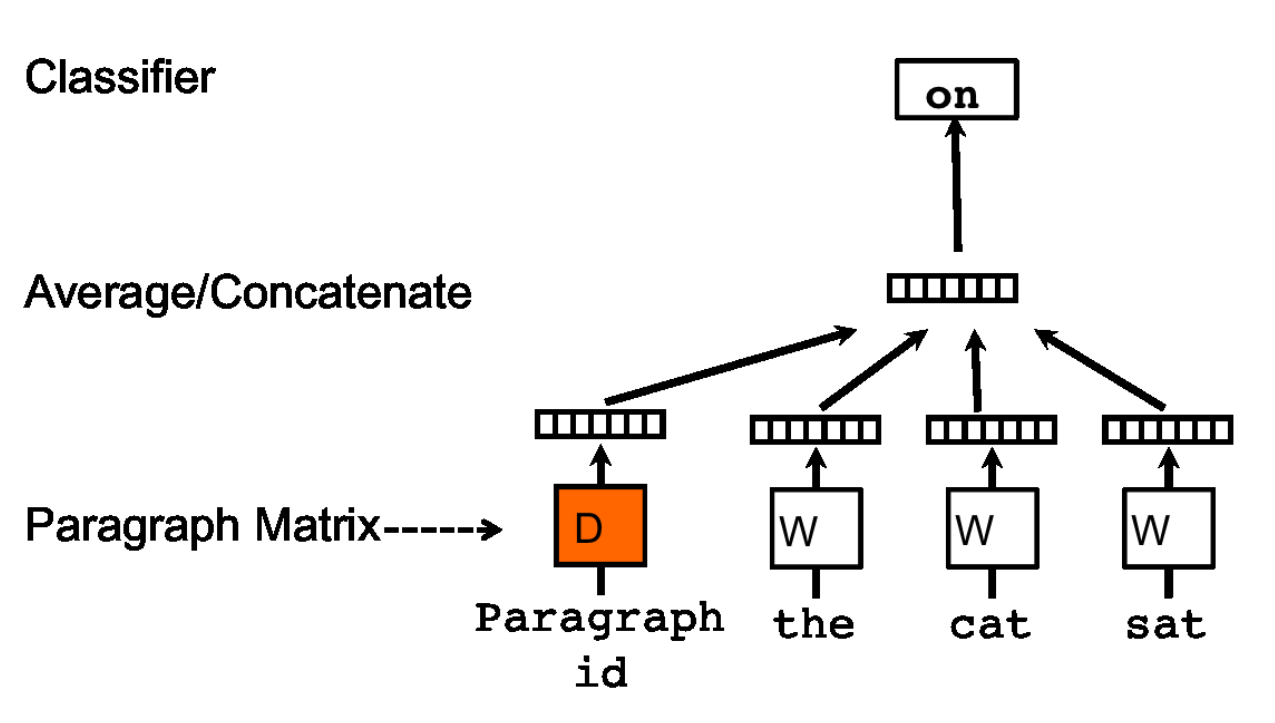
\includegraphics[width=250px]{../chapters/implementation/pics/doc2vec}
	\caption{\label{pic:doc2vec} Visualization of a training step of a Doc2Vec network {\cite{wuWordMoverEmbedding2018}}}
\end{figure}

\subsubsection{Selection of a document embedding technique}

Summarizing the previously discussed methods by three of their main characteristics - number of hyperparameters, maximum processable document length and type of model results in  \autoref{tab:overview_doc_embedding}.
\begin{table}
	\centering
	\begin{tabular}{ c | c | c }
		\hline 
		Technique & Max. document length & Type \\ \hline
		Tf-Idf BOW & unlimited & Probabilistic \\ \hline
		Latent Dirichlet Allocation & unlimited & Probabilistic \\ \hline
		Doc2Vec & unlimited & NN \\ \hline
		Word mover's embedding & unlimited & Kernel method \\ \hline
		BERT & 512 characters & NN \\ \hline
	\end{tabular}
	\caption{\label{tab:overview_doc_embedding} Table summarizing the key features of different document embedding techniques}
\end{table}

The model is now selected by exclusion. Since our database contains documents which are longer than 512 tokens and each token has a length of at least 1 character, BERT is eliminated as a potential document embedding technique. It would be possible to take word embeddings from BERT and average them in order to get a document embedding as it was proposed and further developed in \cite{deboomRepresentationLearningVery2016} for Word2Vec embeddings, but there was no scientific or non-scientific literature that suggested that this works for the case of contextualized BERT embeddings.
Furthermore the previous literature mapping study showed that there is not a lot of work done for explaining probabilistic models or models utilizing kernel tricks, therefore TF-Idf BOW, the LDA and the Word Mover's embedding are not of interest in this case. Only Doc2Vec remains, supporting both an unlimited document length and being of type 'NN' and therefore potentially being able to support at least 7 explainability techniques sourced from the mapping study. Since neural networks are a focus for interpretability research at the moment, as visible in \autoref{fig:applicability_gamut}, this technique is possibly more future-proof in regard to being able to support interpretability techniques which are yet to be developed.

\subsection{Topic extraction}

Currently the only used topic extraction method is the LSA. Since the underlying SVD is a purely linear technique, the questions stands if the results of the topic extraction improve when nonlinear features are taken into account. One technique to perform an nonlinear, unsupervised dimensionality reduction is the \textit{Autoencoder}. This type of neural network consists of an encoder network and a decoder network as seen in \autoref{pic:autoencoder}. The encoder maps an input to an intermediate layer, while the decoder maps a vector from its representation in the intermediate layer to a vector in the vector space of the original input.

The composition of encoder and decoder is then trained to reconstruct the input from its intermediate layer via a standard backpropagation algorithm. Choosing the intermediate layer of lesser dimensionality compresses the input vectors, which constitutes as a dimensionality reduction. As Wang et al. \cite{wangAutoencoderBasedDimensionality2016} pointed out, an autoencoder can emulate the results of a PCA/SVD by choosing a linear activation function for all neurons and may even outperform it for other nonlinear activation functions.

Adding a sparsity constraint to the encoding network can help to describe a project by as little features as possible. Since the features could be interpreted as topics, this constraint helps the clustering task downstream.

\begin{figure}[t]
	\centering
	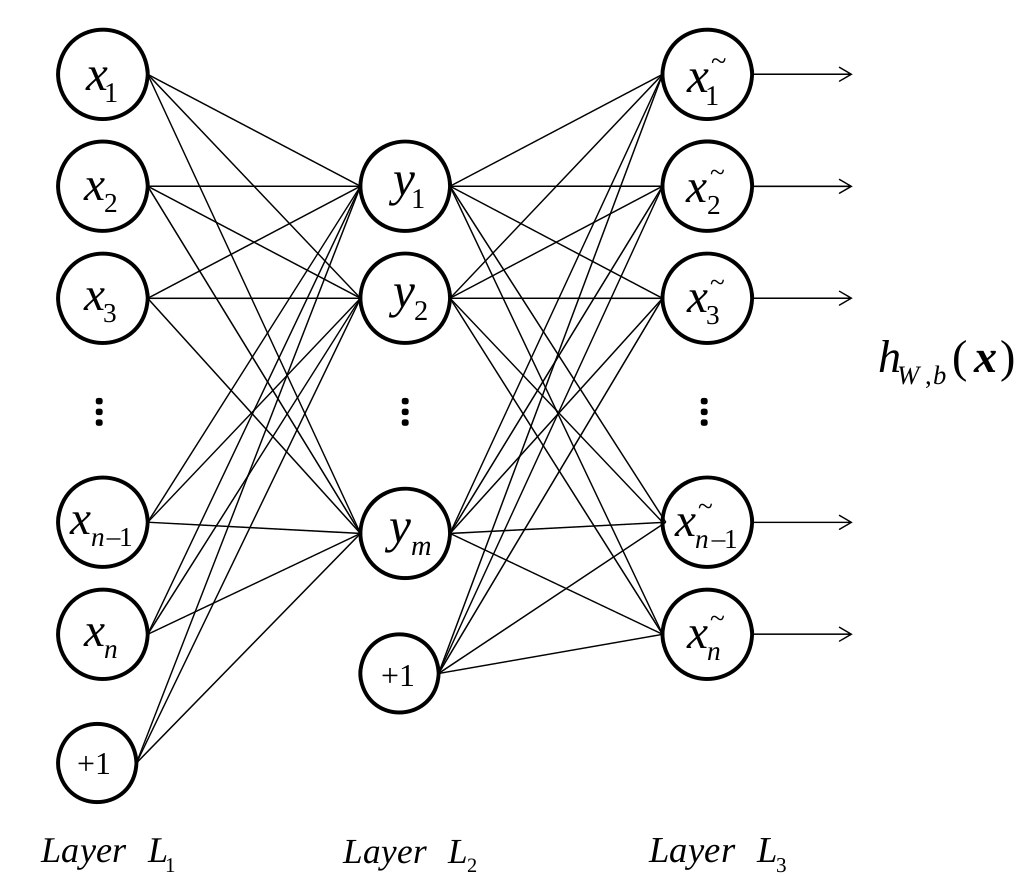
\includegraphics[width=250px]{../chapters/implementation/pics/autoencoder}
	\caption{\label{pic:autoencoder} Strucuture of a simple autoencoder {\cite{wangAutoencoderBasedDimensionality2016}}}
\end{figure} 

Training the model with an embedding dimension of 50, binary crossentropy as a loss function and Adadelta optimizer shows that the model achieves a loss of 0.005 after 75 epochs on the training set and approximately 0.01 on the validation set \autoref{pic:autoencoder_loss}.

\begin{figure}[t]
	\centering
	\includegraphics[width=400px]{/home/tim/HCC/IKON-backend/src/topicextraction/nlp/plots/autoencoder_loss}
	\caption{\label{pic:autoencoder_loss} Graph showing the training and validation loss of the autoencoder over progressing epochs}
\end{figure}

 

\subsection{Clustering}

As described in the beginning of this chapter a K-Means clustering would now classify the documents in the latent topic space. A problem that this approach poses is that the assumption that the Euclidian distance (EuD), which is the inert similarity measure of the K-Means algorithm is meaningful in our vector space may not be true. Another distance measure which may may encode more semantic meaning could be the previously mentioned \textit{Word Mover's Distance}. Since it uses the generated word embeddings and their order in the document to compute distances, it may be more suited for comparing texts and subsequently also yield better results for the clustering. This weighs even heavier if the corpus is vectorized as a sparse matrix since the Euclidian distance, as described in \autoref{chap:introduction}, looses its meaning . In our case, having embeddings from a Doc2Vec model, we don't have to deal with this additional problem, but the question remains if the two distance measures differ on our dataset.  
Comparing the distances between documents generated by both the Word Mover's distance and the Euclidian distance in \autoref{pic:wmd_eud_boxplot} it is apparent that there is indeed a difference. Therefore it is worth investigating if using this information improves the clustering results. 

\begin{figure}[t]
	\centering
	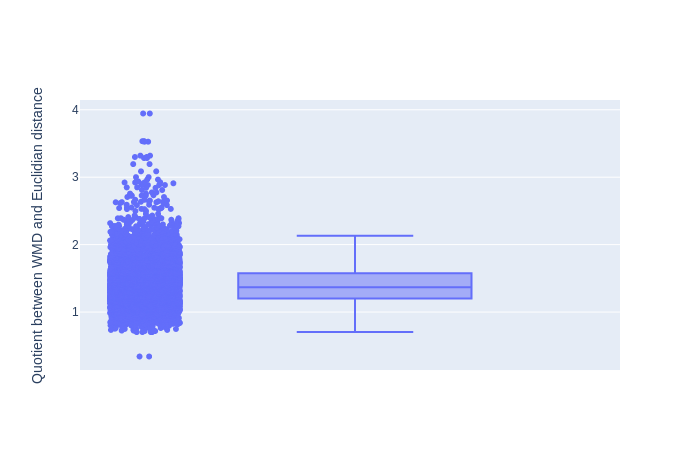
\includegraphics[width=400px]{/home/tim/HCC/IKON-backend/src/topicextraction/nlp/plots/wmd-eud}
	\caption{\label{pic:wmd_eud_boxplot} Boxplot showing the distribution of the quotients between WMD and EuD for all documents}
\end{figure}

Inspired by Liu et al. \cite{Liu:2018:INE:3219819.3220001} I chose a hierarchical clustering approach, specifically \textit{Agglomerative Clustering}, as a contending method to the K-Means algorithm. This method works bottom-up since in the beginning it considers every data point to be its own cluster. Now in every step two clusters are merged which minimize a given linkage metric. The distance calculations between points are performed by a lookup in a precomputed distance matrix which enables the usage of any given distance metric. Doing this until only one cluster remains, creates a binary tree, which describes the hierarchy of the data given the used metric. 

\subsection{Visualization}

In order to visualize all the results from the topic modeling pipeline I developed a D3.js-based interface, which is embedded in the Jupyter notebook in which the code for all the numerical computations resides. Since Jupyter is embracing the browser as a frontend, there is the possibility to embed arbitrary Javascript code in a cell and inject any kind of visualization. In order to do that I construct a JSON object containing all the results from the topic pipeline (vectorized documents as scatter points and linearized points, top words, the interpolated topography, model parameters etc.) and pass it into the Javascript code via Jupyter's $Javascript$ function and string interpolation which renders it in the browser.

The interface consist of a discrete slider controlling the granularity of the clustering, which translates to the number of clusters which are computed in the topic modeling pipeline. Furthermore there is a dropdown selection where one can switch between the scatter and the linearized variants of the scatter plots.
Beneath the parts of the interface which are connected to parameter selection, the top words for all clusters are displayed and even further down the plot is located in which each project is visualized as a circle. Changing any of these parameters result in an immediate change of the computed plot and the top words. Additionally one can hover over projects in order to reveal additional metadata about the project (project ID, title, top words).

\begin{figure}[t]
	\centering
	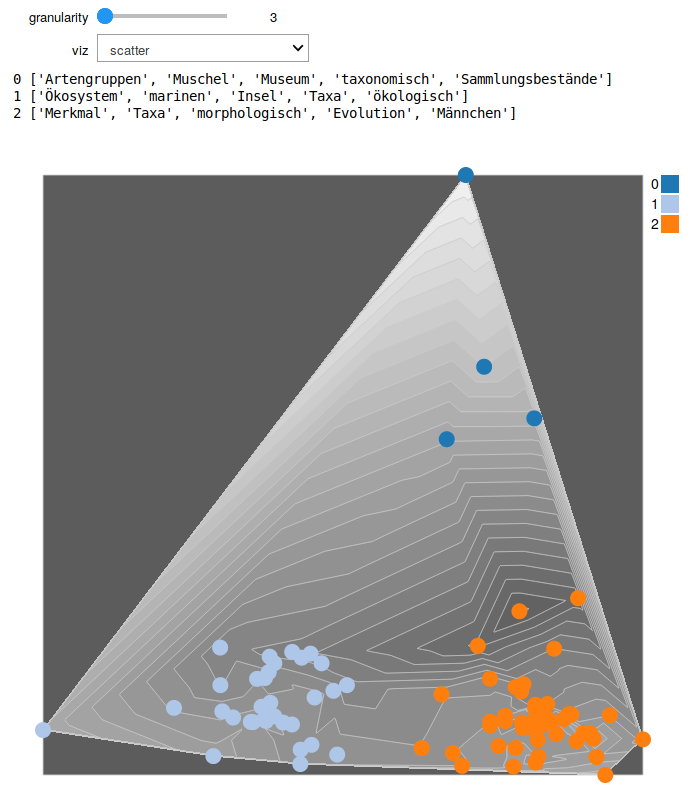
\includegraphics[width=300px]{../chapters/implementation/pics/interface}
	\caption{\label{pic:interface} Screenshot showing the exemplary interface}
\end{figure}

